\subsection{Bipartite graphs and matchings}

The rules at the heart of this paper come from a basic idea in graph theory. We first state it in general, then show
how a band of a Sudoku becomes one of these graphs.

\begin{figure}[H]
\centering
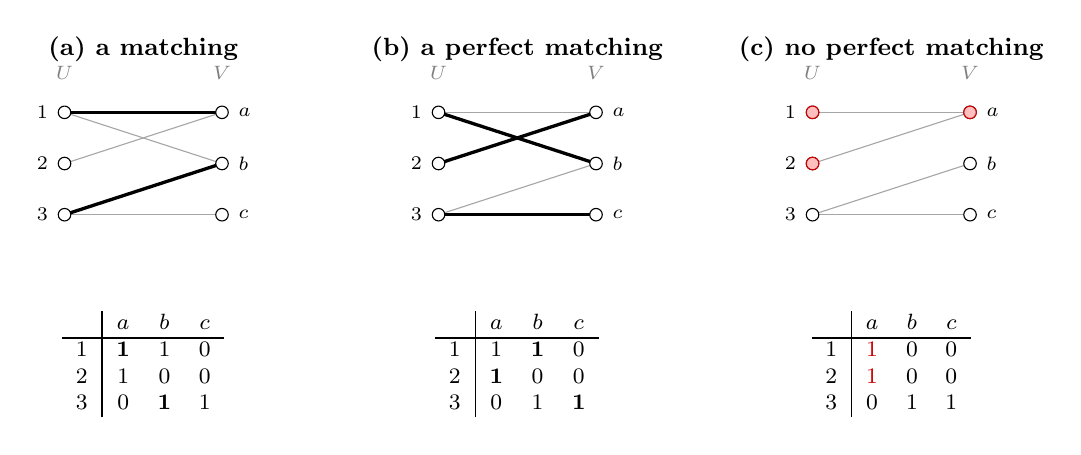
\begin{tikzpicture}[x=0.5cm,y=0.5cm,
  vtx/.style={circle,draw,fill=white,inner sep=1.6pt},
  bad/.style={circle,draw=red!80!black,fill=red!25,inner sep=1.6pt},
  edge/.style={gray!70,thin},
  pick/.style={very thick}]
  \foreach \p/\title/\X in {0/{(a) a matching}/0, 1/{(b) a perfect matching}/9.5, 2/{(c) no perfect matching}/19} {
    \node[font=\small\bfseries] at (\X+2,4.6) {\title};
    \node[font=\scriptsize,gray] at (\X,4.0) {$U$};
    \node[font=\scriptsize,gray] at (\X+4,4.0) {$V$};
  }
  % (a), (b): the graph of the worked example; (c): 1 and 2 are both joined only to a
  \foreach \X/\nm in {0/a,9.5/b,19/c} {
    \foreach \i in {0,1,2} {
      \coordinate (\nm s\i) at (\X,3-1.3*\i);
      \coordinate (\nm p\i) at (\X+4,3-1.3*\i);
    }
  }
  \foreach \nm in {a,b} \foreach \i/\j in {0/0,0/1,1/0,2/1,2/2} \draw[edge] (\nm s\i) -- (\nm p\j);
  \foreach \i/\j in {0/0,1/0,2/1,2/2} \draw[edge] (cs\i) -- (cp\j);
  \foreach \i/\j in {0/0,2/1} \draw[pick] (as\i) -- (ap\j);
  \foreach \i/\j in {0/1,1/0,2/2} \draw[pick] (bs\i) -- (bp\j);
  \foreach \nm in {a,b,c} \foreach \i in {0,1,2} {
    \node[vtx,label={[font=\scriptsize]left:$\the\numexpr\i+1\relax$}] at (\nm s\i) {};
    \node[vtx,label={[font=\scriptsize]right:$\ifcase\i a\or b\or c\fi$}] at (\nm p\i) {};
  }
  \foreach \i in {0,1} \node[bad] at (cs\i) {};
  \node[bad] at (cp0) {};
  % biadjacency matrices
  \node[font=\footnotesize] at (2,-3.4) {$\begin{array}{r|ccc}
      & a & b & c \\ \hline
    1 & \mathbf{1} & 1 & 0 \\
    2 & 1 & 0 & 0 \\
    3 & 0 & \mathbf{1} & 1
    \end{array}$};
  \node[font=\footnotesize] at (11.5,-3.4) {$\begin{array}{r|ccc}
      & a & b & c \\ \hline
    1 & 1 & \mathbf{1} & 0 \\
    2 & \mathbf{1} & 0 & 0 \\
    3 & 0 & 1 & \mathbf{1}
    \end{array}$};
  \node[font=\footnotesize] at (21,-3.4) {$\begin{array}{r|ccc}
      & a & b & c \\ \hline
    1 & \textcolor{red!80!black}{1} & 0 & 0 \\
    2 & \textcolor{red!80!black}{1} & 0 & 0 \\
    3 & 0 & 1 & 1
    \end{array}$};
\end{tikzpicture}
\caption{Matchings in a bipartite graph with $U=\{1,2,3\}$ and $V=\{a,b,c\}$ (top), each with its biadjacency
matrix (bottom). Every matching is a subset of the graph's edges; each panel draws one such subset with thick edges
and bold 1s, and the other edges thin and gray. (a) One of several matchings of this graph, $\{1a,3b\}$: no vertex is
used twice, but $2$ and $c$ are left out, and it cannot be extended, since $2$'s only neighbour $a$ is taken. (b) The
same graph's only perfect matching, $\{1b,2a,3c\}$, so here nothing is chosen: $2$ must take $a$, then $1$ must take
$b$ and $3$ must take $c$. Every vertex is used once, and the bold 1s form a permutation matrix. (c) A graph with no
perfect matching, so nothing is drawn thick: $1$ and $2$ are both joined only to $a$ (column $a$ holds both of their
1s), so one of them is always left out.}
\label{fig:matching}
\end{figure}

\paragraph{The general idea.} A \emph{bipartite graph} has two separate sets of vertices, $U$ and $V$, and edges
that each join a vertex of $U$ to a vertex of $V$; no edge joins two vertices of the same set. Each edge is a pair
$(u,v)$ with $u\in U$ and $v\in V$, so the edge set $E$ is a subset of $U\times V$. A \emph{matching} is a set of edges
no two of which share a vertex. A \emph{perfect matching} is a matching that uses every vertex exactly once. Since each
edge uses one vertex from each side, a matching of $m$ edges uses $m$ vertices of $U$ and $m$ of $V$, so a perfect
matching can only exist when $|U|=|V|$; a matching in general needs no such thing. Take $U=\{1,2,3\}$ and
$V=\{a,b,c\}$. A one-to-one pairing of $U$ with $V$ is a bijection $f\colon U\to V$, which we identify with its three
pairs $(1,f(1)),(2,f(2)),(3,f(3))$. To count them, ignore $E$ for a moment: $f(1)$ has 3 choices, $f(2)$ then has 2 (it
must differ from $f(1)$), and $f(3)$ has 1, so there are $3\cdot 2\cdot 1=3!=6$ pairings. A perfect matching of the
graph is one of these six whose three pairs all lie in $E$ (\cref{fig:matching}). An edge \emph{lies on a perfect
matching} when at least one perfect matching includes it. An edge that lies on no perfect matching can never be part
of a complete assignment, however the rest is chosen, so it can be deleted.

A small bipartite graph can be written as a table of 0s and 1s, its \emph{biadjacency matrix} $A$: one row for each
vertex of $U$, one column for each vertex of $V$, and $A_{uv}=1$ when $u$ and $v$ are joined. An ordinary
\emph{adjacency matrix} has a row and a column for every vertex of the graph, $6\times 6$ here; for a bipartite graph
it has the block form $\bigl(\begin{smallmatrix} 0 & A \\ A^{\mathsf T} & 0 \end{smallmatrix}\bigr)$, since no edge
joins two vertices of the same side, so $A$ alone holds the whole graph. (``Bi'' because its rows and columns are
indexed by the two different sets.) $A$ is $|U|\times|V|$, so in general it need not be square. A matching is a set of
1-entries of $A$ with at most one in each row and at most one in each column. A perfect matching needs exactly one in
every row and every column, which is possible only when $A$ is square, $|U|=|V|$, as shown above. Such a pattern, a
square 0-1 matrix with exactly one 1 in each row and each column, is a \emph{permutation matrix}: it is the identity
matrix with its rows reordered, and the $3!=6$ permutation matrices of size 3 are the six pairings. So a perfect
matching of the graph is a permutation matrix $P$ that fits inside $A$, meaning $A_{uv}=1$ wherever $P_{uv}=1$. Every
graph in this paper is three against three, so its table is $3\times 3$. The whole graph is then 9 bits, one per entry of $A$, so there
are only $2^9=512$ possible graphs, and reading the 9 bits as a binary number gives each graph an index from 0 to 511.
Once, before solving starts, we build a table of 512 entries: the entry at index $A$ is another 9-bit pattern, with a
1 exactly at the entries of $A$ that lie on some perfect matching. A $3\times 3$ graph can have anywhere from zero to
six perfect matchings, and the entry is all of them laid on top of each other. When every entry of $A$ is 1, all six
pairings fit, every edge lies on one, and the entry equals $A$. The graph of \cref{fig:matching}(b) has exactly one, so
its entry is just the three bold 1s. The worked example below has two, so its entry is the union of their six 1s,
which may overlap. The graph of \cref{fig:matching}(c) has none, so its entry is all 0s. During the solve, the solver builds $A$ from
the current candidates and reads the table at index $A$. Every 1 of $A$ that is 0 in the entry is an edge on no
perfect matching, so it is deleted; an all-zero entry means the current position cannot be completed, so the last
guess was wrong. Working this out directly would mean trying the six pairings against $A$ every time, with branches
on the results; the table does that work once for all 512 graphs, so at solve time it is a single memory read.

\paragraph{From a band to a bipartite graph.} Fix one digit, say 5, and one band. The rules of Sudoku say that in the
finished grid 5 appears exactly once in each of the band's three rows, and exactly once in each of its three boxes.
Build the bipartite graph whose first set is the band's three rows and whose second set is its three boxes, with an
edge from row $r$ to box $k$ when 5 is still a candidate somewhere in the triad where row $r$ crosses box $k$. Then:
\begin{itemize}
\item The three 5s of the finished band sit in three triads. ``Once per row'' means each row vertex is used by
  exactly one of them, and ``once per box'' means each box vertex is used by exactly one. So the three triads that
  hold the 5s form a perfect matching of this graph, and it uses only existing edges, because the 5s must be at
  candidates.
\item Conversely, every perfect matching is a way the rows could share out the boxes.
\item So a triad whose edge lies on no perfect matching cannot hold the 5, and 5 can be removed from all three of its
  cells. This is the \emph{band rule}.
\end{itemize}
The biadjacency matrix is the $3\times 3$ table with $A_{rk}=1$ when 5 has a candidate in row $r$, box $k$. In the solver
these 9 bits are computed directly from the digit's 27-bit band mask, and they are the index into the lookup table.

\paragraph{A worked example.} Suppose that in some band, 5 can still go in boxes 0 and 1 of row 0, boxes 0 and 1 of
row 1, and all three boxes of row 2 (\cref{fig:band}). The biadjacency matrix, with rows of the table for the rows of
the band and columns for the boxes, is
\[
A = \begin{pmatrix} 1 & 1 & 0 \\ 1 & 1 & 0 \\ 1 & 1 & 1 \end{pmatrix}
\qquad\longrightarrow\qquad
\begin{pmatrix} \mathbf{1} & \mathbf{1} & 0 \\ \mathbf{1} & \mathbf{1} & 0 \\ 0 & 0 & \mathbf{1} \end{pmatrix}.
\]
Rows 0 and 1 can each use only boxes 0 and 1, so between them they use up both, and row 2 must take box 2. Two
permutations fit: row 0 $\to$ box 0, row 1 $\to$ box 1, row 2 $\to$ box 2, and row 0 $\to$ box 1, row 1 $\to$ box 0,
row 2 $\to$ box 2. The table entry is their union, shown on the right: each 1 of rows 0 and 1 lies on one of the two,
but $A_{20}$ and $A_{21}$ lie on neither, so 5 is removed from the triads of row 2 in boxes 0 and 1, even though
nothing inside those triads ruled it out.

\paragraph{What familiar techniques look like in this picture.} A human solver would reach the same conclusion in
steps: ``in row 1 the 5 must be in box 0, so box 0's 5 is in row 1, so row 0 can't have its 5 in box 0'', and so on.
Several named techniques are single cases of the matching test. If a row has candidates in only one box, that box
belongs to that row (a locked-candidate deduction), and the other rows lose that box. If two rows of the band have
candidates only in the same two boxes, those two boxes are used up by them, so the third row must use the third box;
that is the worked example above.
Hall's theorem~\cite{hall1935representatives} captures all of these at once: a perfect matching exists exactly when
every set of $k$ vertices on one side is joined to at least $k$ vertices on the other. The table does the whole
analysis in one lookup instead of a chain of named steps.

\paragraph{What the graph leaves out.} The graph only records \emph{whether} a triad still holds a candidate, not in
which of its three columns. So the band rule removes whole triads and never chooses between the cells of one; the
columns are handled by the next rule and by the other constraints.

\paragraph{The stack version.} Turn the picture sideways. In a stack, 5 appears once in each of the stack's three
columns and once in each of its three boxes, and the three boxes of a stack lie in the three different bands, so
``once per box'' is the same as ``once per band''. The bipartite graph now has the three bands on one side and the
stack's three columns on the other, with an edge from band $b$ to column $c$ when 5 is still a candidate in column $c$
within band $b$. The finished grid's three 5s in the stack again form a perfect matching, so any (band, column) edge on
no perfect matching can be deleted: 5 is removed from that column in that band. This is the \emph{stack rule}. For
example, if in one stack 5 can be in columns $\{0,1\}$ in band 0, only column 0 in band 1, and any column in band 2,
then band 1 takes column 0, band 0 must take column 1, and band 2 column 2: three of the six edges are deleted. The
solver uses the same 512-entry table as for the band rule.

\paragraph{The general principle.} The same reasoning applies to any Sudoku unit: in a row, the nine cells must be
paired one-to-one with the nine digits, which is a perfect matching in a $9\times 9$ bipartite graph of cells and digits.
R\'egin's filtering algorithm for \texttt{alldifferent} constraints~\cite{regin1994filtering} deletes every edge of such
a graph that lies on no perfect matching, using an efficient matching algorithm, and constraint solvers use it for
Sudoku~\cite{simonis2005sudoku}. Our rules apply the same principle to much smaller graphs, three against three, which
is small enough to precompute every case and apply it with one table lookup.

Finally, a \emph{template} is one complete way of placing a single digit nine times, once in every row, column and
box. There are 46{,}656 templates; \cref{sec:negative} tests a solver built on them.

